%!TEX root = thesis.tex

\chapter{Evaluation}
\label{ch:evaluation}

\section{Challenges for evaluation}
\label{sec:eval-challenges}
Different researchers use different metrics to evaluate the performance of their agents. 
There are multiple factors that increase the difficulty of properly evaluating the performance.

\subsection{Randomness of battles}
\label{sec:eval-challenges-randomness}
As teams are generated randomly, one player often ends up with a slightly better team than his opponent.
In extreme cases, one player may not even have a chance at winning the battle. While battling
our agent during the evaluation process, one particular game stood out as the first Pokémon of 
\textbf{Player1} was capable of defeating the entire enemy team. \\
The Pokémon of \textbf{Player1} was a \textit{Volcarona} with the following moves:
\begin{itemize}
    \item \textit{Fire Blast}, a damaging \textit{Fire}-Type move
    \item \textit{Quiver Dance}, a \textit{Bug}-Type move that boots the users \ac{SPA}, \ac{SPD} and 
    \ac{SPE} by one stage each.
    \item \textit{Bug Buzz}, a damaging \textit{Bug}-Type move
    \item \textit{Roost}, a move that restores half of the user's maximum \ac{HP}
\end{itemize}
This Pokémon was able to defeat the entire enemy team with little to no possible counter play:
The first enemy Pokémon, \textit{Leafeon}, a \textit{Grass}-Type Pokémon was killed in one hit using
\textit{Fire Blast} after damaging \textit{Volcarona} using \textit{X-Scissor}. \\
Next, \textit{Glalie}, an \textit{Ice}-Type was sent into battle. \textit{Glalie} uses his best move,
\textit{Earth Quake} which brings \textit{Volcarona} to 52\% \ac{HP}. As the enemy does not prose much thread to 
\textit{Glalie}, \textbf{Player1} decided to boost using \textit{Quiver Dance}. Now, \textit{Volcarona}
is faster than his enemy and kills it again in one hit using \textit{Fire Blast}. \\
Then, \textit{Mr. Mime (Galar)} is sent into battle. He fails to pressure \textit{Volcarona} and therefore,
\textbf{Player1} can heal his Pokémon using \textit{Roost} and further boost using \textit{Quiver Dance}. After
defeating \textit{Mr. Mime (Galar)}, \textit{Volcarona} is back to 84\% HP and boosts of 2.5 \ac{SPA},
1.5 \ac{SPD} and 2.5 \ac{SPE}. 
Boosted this high, \textit{Volcarona} can one-shot both the enemy \textit{Volcarona},
\textit{Pheromosa} and the dynamaxed \textit{Scraggy} using \textit{Fire Blast}. \\
To eliminate the impact of these extreme cases, evaluation of agents against other agents 
should be done using multiple hundreds to thousands of games against each other. \\
In order to quantify and better visualize the randomness of battles, over 70,000 \ac{GEN8RANDBATS}
were generated, and the team information was stored. Next, the board rating was calculated. Let $e$ be 
a Pokémon and $C$ the set of all enemy Pokémon that are countered by $e$. We compute the score of 
a team member $e$ as follows: 
\begin{equation}
  \text{member-score (Pokémon: e)} = \sum_{j \in C} 1
\end{equation}
The score of a team $p$ is defined by:
\begin{equation} 
  \text{team-score (Team: p)} = \sum_{e \in p} \text{member-score}(e)
\end{equation}
Finally, the board rating of two teams $p_1$ $p_2$ is defined as the difference between their respective 
team score
\begin{equation}
  \text{board rating (Team: $p_1$, Team: $p_2$)} = \text{team-score($p_1$)} - \text{team-score($p_2$)}
\end{equation}
Therefore, a low board rating indicates that the player has fewer counters than his opponents. Finally,
the generated games were played out by \textit{Random}-Player as well as \textit{MaxDamage}-Player. The 
win-rate of both agents at a given board rating is displayed in figure~\ref{fig:wr-board-rating}. 
\begin{figure}[h]
	\centering
	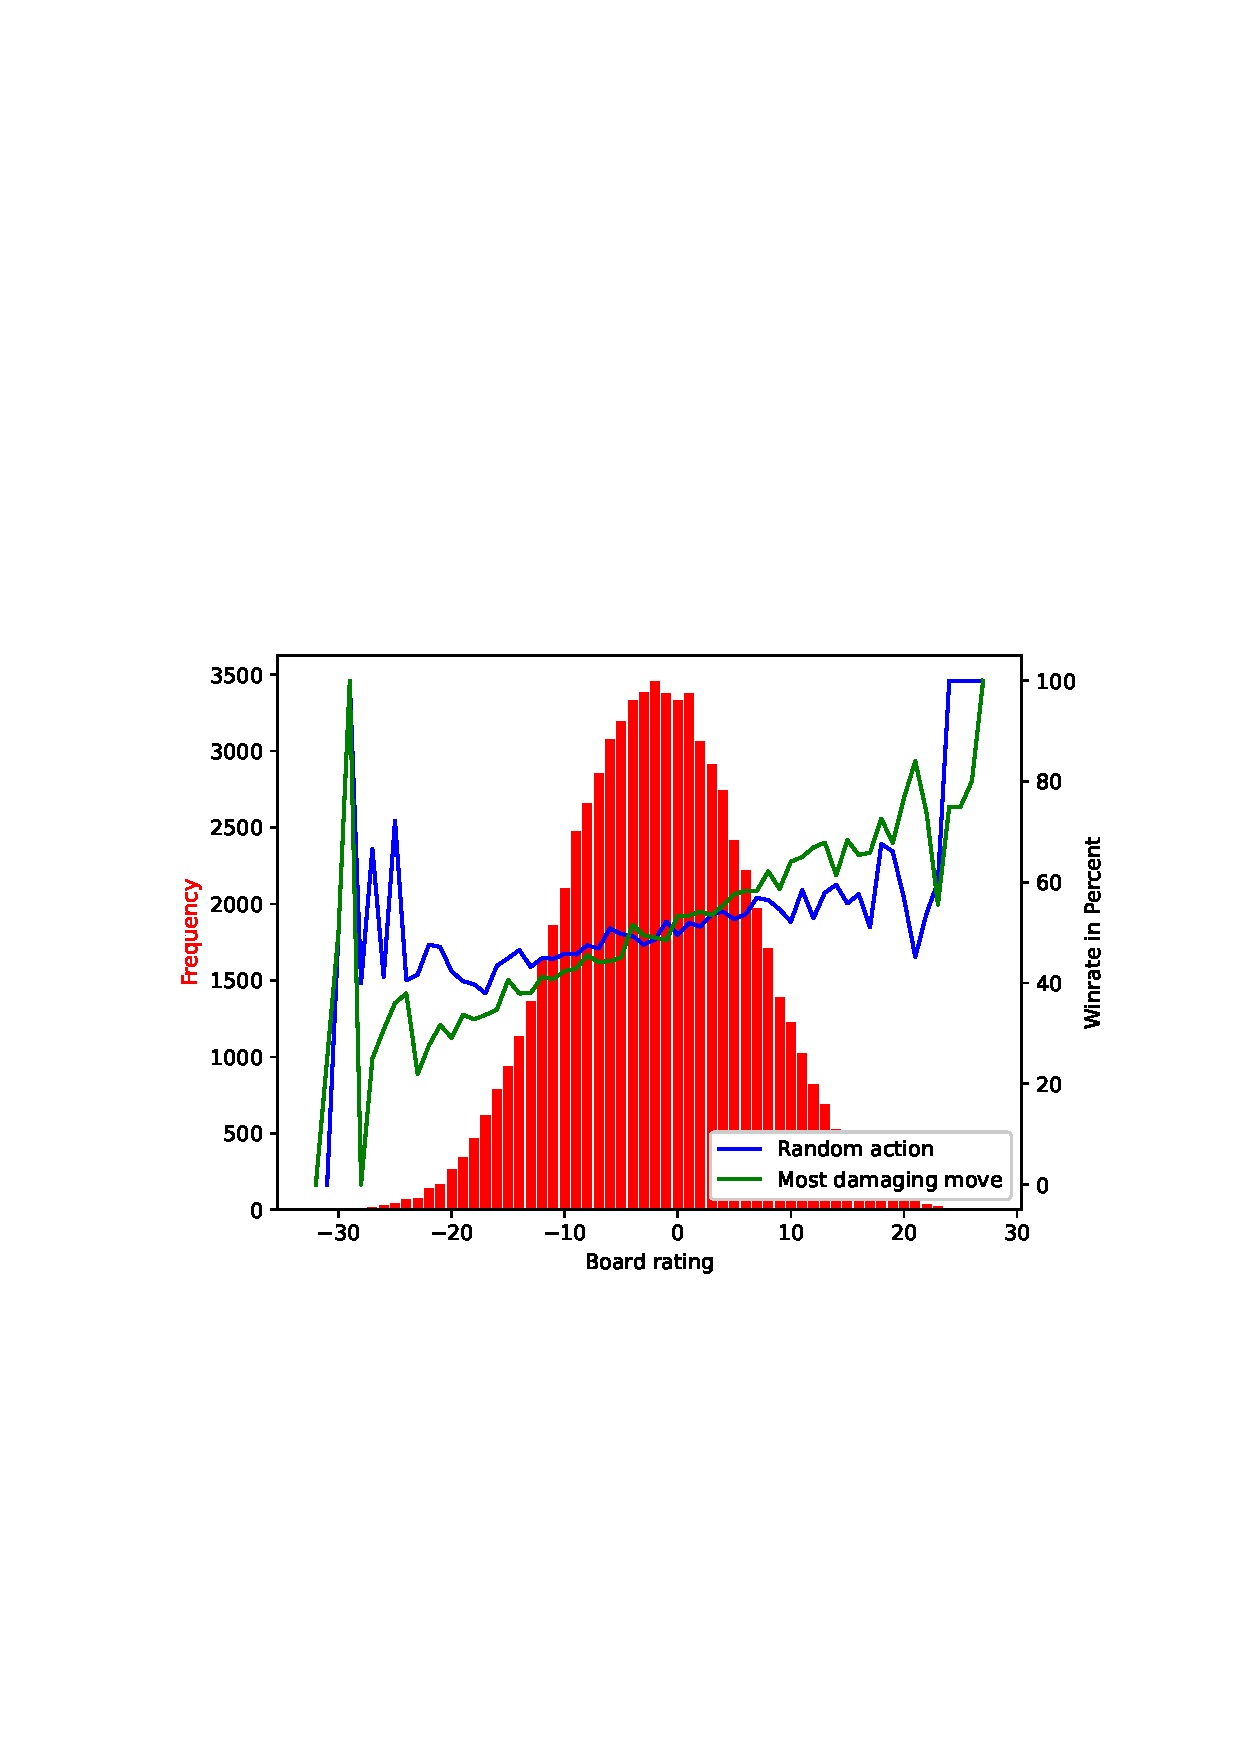
\includegraphics[width=\textwidth]{images/boardrating.pdf}
	\caption{Win rate of the baseline agents at a given board rating. Both agents
  move have a lower win rate on unfavorable board ratings while winning more games on a positive rating.}
	\label{fig:wr-board-rating}
\end{figure}
Most notably, fair games, meaning games with a board rating close to zero, are gaussian-distributed with the majority
of the matchups being almost fair according to our metric. The blue line indicates the win rate of a \textit{Random}-Player
when playing against another \textit{Random}-Player at the given board rating, indicated green is the win rate of two
\textit{MaxDamage}-Players. There are multiple important observations: Firstly, at negative board ratings, both
agents have a significantly lower win rate against the opponent while positive board ratings indicate a high chance of 
winning. Despite collecting over 70,000 data points, board ratings worse than $-20$ or better than $+20$ will be ignored in this analysis
as the large irregularities in these areas indicate an insufficient amount of data points. 
The steeper slope of the green line is likely explained by the \ac{RNG} of the actions performed by random agents having 
a much higher influence than the actual team composition. As a random agent rarely makes the correct choice, it 
fails to utilize the full potential of a stronger team. 
\todo{More refined metric: Same results, longer to simulate as better agents required. Showdown replays do not contain
all information neccesary.} 

\subsection{Evaluation against human opponents}
As described in section~\ref{sec:showdown-background}, Pokémon Showdown allows researchers to use bots on the
ranked ladder. 

\section{Agents}
During this thesis, two different agents were developed, \textit{HerrDonner} and \textit{HerrGewitter}.

\subsection{HerrDonner}
This agent was designed to establish a good baseline and to demonstrate the capabilities of a very
simple rule set. The agent is capable of looking multiple turns into the future. To determine
what moves to be used, the Agent generates every possible move combination with the specified amount
of turns into the future and calculates the expected outcome while assuming that the enemy does 
not move at all, similar to the \ac{BFS}-based algorithm described in paragraph \ref{sec:related-bfs}. 
No drawback moves that heal the agent, set hazards or field conditions or inflict status conditions
are not considered unless they result in the highest amount of damage dealt. Also, stat changes are 
not taken into account, neither for damage calculation nor for rating of matchups. 
This results in the bot often spamming moves like \textit{Draco Meteor}, a \textit{special} 
\textit{Dragon}-type move that deal a lot of damage but also lower the
users \ac{SPA} by two stages resulting in the move dealing less damage every time it is carried out. 
When the agent is forced to switch, it will switch to a check if available. If no check is available,
a counter is sent into battle if one exists. Otherwise, a random Pokémon will be picked. \\
At the start of each turn, \textit{HerrDonner} will check if the current matchup is not favorable, 
a matchup is deemed unfavorable, if the current Pokémon is neither check nor 
counter to the current enemy. On a bad matchup, the bot will switch to an available 
check or counter. If neither is available, the bot won't switch and try to
defeat the current opponent with his active team member. \\
Dynamaxing is implemented in a very simple and naive way: The agent will always dynamax the
active Pokémon as soon as more than four enemy Pokémon are known. Lastly, if the
current Pokémon is dynamaxed, the agent will not switch, even if the current matchup is not
favorable. The challenges of properly using this mechanic will be explained in~\ref{par:eval-dynamx}.

\subsection{HerrGewitter}
\label{sec:HerrGewitter}
\textit{HerrGewitter} behaves like described in section \ref{ch:approach}. Here, the most notable
differences between both agents are highlighted, and limitations of this agent are discussed. \\
Firstly, \textit{HerrGewitter} takes more factors into consideration. Now, damage calculation is done
in regards to current stat changes and status conditions. Additionally, abilities and items are taken 
into account. Furthermore, recoil from moves, healing both from items
like \textit{Leftovers}~\autocite{Bulbapedia:Leftovers} and moves like \textit{Recover} are not neglected
anymore. \\
Switching and the selection of moves is done as described in section~\ref{ch:approach}. \\
These improvements lead to \textit{HerrGewitter} avoiding mistakes of \textit{HerrDonner}. For example,
this agent will burn a physical attacker using \textit{Will-O-Wisp}~\autocite{Bulbapedia:WillOWisp}
in order to reduce damage taken over the next turns. The agent will also boost and heal itself in favorable
situations which stalls the game and forces the opponent to react. Another major improvement is that the
agent switches out the current Pokémon if stat changes resulted in an unfavorable matchup which is especially
important as stat changes reset on a swap. However, there are still a lot of features that \textit{HerrGewitter} 
is lacking. 

\paragraph{Weather and Field effects}
One such feature is a proper support for weather and field effects in the damage calculation as well
as in the \textit{MiniMax}-Algorithm. For instance, a consequence of this is the agent lacking awareness
of the fact that a \textit{Fire}-Type move deals 1.5 more damage during \textit{Harsh Sunlight}.

\paragraph{Hazards}
Currently, the agent will always try to set a non-present Hazard in the early game as this usually 
results in a long term benefit. There are however some notable exceptions to this that 
are not yet implemented:
\begin{itemize}
  \item The agent will always set as many hazards as possible in the early game, even if the current matchup 
  is unfavorable, including always setting up to two layers of spikes. A small test on human players indicated
  that this leads to slightly better results than only setting hazards on good matchups, but due to the very
  small sample size, future work is needed to determine the best strategy for setting hazards.
  \item The agent does not take the damage taken by hazards into account when switching Pokémon. 
  \item The agent will always use \textit{Toxic Spikes} even if the opponent has a \textit{Poison}-Type
  Pokémon on his team that will remove this hazard upon being switched in.
  \item The agent will use Hazards even if the current enemy is known to have a hazard-clearing move like
  \textit{Defog}~\autocite{Bulbapedia:Defog}
  \item The agent will not clear hazards
\end{itemize}

\paragraph{Choice Items}
As mentioned in section \ref{sec:Important-items}, Pokémon holding a \textit{Choice}-item are locked into using always 
the same move until they are switched out. The agent has two major flaws in regard to these items: When the active
Pokémon of the agent is holding a choice item and is already locked into a move, the agent is not aware of the fact that
once the Pokémon is switched out, it will regain access to his other moves which leads to an incorrect prediction
for future matchups. As described in section~\ref{sec:determine-matchups}, the only matchups re-evaluated
on a given turn are matchups that include one of the currently active Pokémon. The following example illustrates how
this design decision leads to issues on Pokémon with \textit{Choice}-items: \\
In the given scenario, our agent has an active \textit{Garchomp} which is locked into using \textit{Earth Quake}. The 
\textit{Garchomp} also has access to the \textit{Rock}-Type move \textit{Stone Edge}. This turn \textit{Butterfree},
a \textit{Bug / Flying}-Type Pokémon
is sent into Battle. As the \textit{Ground}-Type move \textit{Earth Quake} has no effect on \textit{Butterfree}, the agent will
switch out \textit{Garchomp} for another Pokémon. In the current implementation, matchups for \textit{Garchomp} are not
re-evaluated. While this won't lead to problems in the early game, this results in an incorrect \textit{MiniMax} calculation
as for matchups involving \textit{Garchomp} and any non-active opponent, \textit{Garchomp} is still assumed to only have
access to the move \textit{Earth Quake}. In this scenario, the agent would fail to realize that \textit{Garchomp} also
has access to \textit{Stone Edge} and would incorrectly assume \textit{Garchomp} to lose all matchups against \textit{Flying}-Type
Pokémon. \\
While this behavior rarely effects battle, the agent failing to notice that an enemy is choice-locked has more often a 
negative impact on the battle: If the enemy is known to be choice-locked into \textit{Earth Quake} we can safely switch 
a \textit{Flying}-Type into battle. This applies especcially if the enemy Pokémon is known to have the \textit{Rock}-type 
super effective
move \textit{Stone Edge} as the enemy can not use this move until switched out and back in again. In this scenario, the
agent wrongfully would not prefer to switch in a \textit{Flying}-Type Pokémon due to the thread posed by 
\textit{Stone Edge}. Switching in a Pokémon resisting \textit{Earth Quake} in this scenario forces the enemy to switch
to another Pokémon. This gained turn advantage can either be used to land an extra move on the next opponent, set hazards,
beneficial field conditions, inflict status conditions or boost the current Pokémon.

\paragraph{Damage Calculator}
The current implementation relies on the Pokémon Showdown Damage Calculator. As of now, this open source project does 
only support direct damage dealt by attacking and lacks functionalities like recoil, healing from items and moves. While
we added these features to our implementation, some moves are still not properly implemented. For example, the move
\textit{Counter} has a move priority of $-5$ and works as follows:
If the last mount of damage dealt before the use of \textit{Counter} is greater than zero and was dealt by a 
\textit{Physical}-Type move, \textit{Counter} will do twice as much damage to the opponent. Otherwise, the move
will miss. Additionally, \textit{Counter} has a lot of extra rules regarding other special moves in place 
~\autocite{Bulbapedia:Counter}. Issues like these are especially obvious on \textit{Wobbuffet} as all of his four
most likely moves, \textit{Mirror Coat}, \textit{Encore}, \textit{Counter} and \textit{Encore} are very useful
yet do not deal any damage and are not implemented yet which leads the agent to believe that this Pokémon is bad 
in every possible matchup and has no good use scenarios whatsoever.

\paragraph{Dynamaxing}
\label{par:eval-dynamx}
As previously stated, dynamaxing is a very complex mechanic that requires sophisticated long term planning for
proper usage. According to \textit{Memezboi69}, the safest usage of this mechanic is to dynamax in a late stage
of the game on a good matchup. He stated multiple reasons for this: \\
Dynamaxing at a later stage of the game reduces the likeliness of an opponent being able to properly react due to the 
limited amount of Pokémon alive. \\
Another flaw of \textit{HerrGewitter} is the fact that defensive dynamaxing is not yet taken into consideration. 
If the opponent dynamaxes offensively, a good way to minimize damage received when no counter is available, is dynamaxing
defensively and using the move \textit{Max Guard} which protects the user from moves. If a Pokémon has access to 
a status move, this move will be replaced by \textit{Max Guard} when dynamaxing. Lastly, dynamaxing can under 
some circumstances also be used in an earlier stage of the game if the current matchup is favorable. 

\paragraph{Predictions}
\label{par:predictions}
When play testing the bot, predictions were noticeable but only seemed to occur rarely. This is 
likely caused by the optimal move against the current Pokémon being equal to the best attack
targeting the predicted switch. In order to compete with higher ranked players, more investigation
on the prediction routine is required. Future work could also include switching in anticipation
of the opponent withdrawing his active Pokémon.

\paragraph{Other special cases}
This list contains more currently unhandled cases which will be addressed in future versions:
\begin{itemize}
  \item The Pokémon \textit{Ditto} can transform itself into the Pokémon of the current opponent.
  \item The Pokémon \textit{Zoroark} can transform itself into another team member. 
  \item The ability \textit{Trace} changes the ability of a Pokémon to the ability of his opponent.
\end{itemize}

\paragraph{MiniMax}
The \textit{MiniMax}-Algorithm described in paragraph \ref{sec:defeat-phase} only supports changes in health
but ignores other important factors such as boosts and status conditions. Therefore, the agent will 
not recognize the possibility to weaken a very strong physical attacker like \textit{Garchomp} by burning
it first and then defeating it with another Pokémon. A simple way to include \ac{BRN} into this algorithm
is to multiply the expected damage dealt by a burned Pokémon with $0.5$. 

\section{Results}
\subsection{Ranked results}
\begin{figure}[h]
  \centering
  \begin{minipage}{.5\textwidth}
    \centering
    \includegraphics[width=1\linewidth]{images/Donner-Elo-Time.png}
    \captionof{figure}*{\textit{HerrDonner}}
  \end{minipage}%
  \begin{minipage}{.5\textwidth}
    \centering
    \includegraphics[width=1\linewidth]{images/Gewitter-Elo-Time.png}
    \captionof{figure}*{\textit{HerrGewitter}}
  \end{minipage}
  \captionsetup{justification=centering,margin=1cm}
  \caption{Elo of \textit{HerrDonner} and \textit{HerrGewitter} after playing 1400 ranked games respectively}
  \label{fig:donner-gewitter-elo}
\end{figure}
Both agents were evaluated at the same time over the span of multiple days by playing over 1400 ranked games each 
against human opponents on Pokémon Showdown. Figure~\ref{fig:donner-gewitter-elo} shows the Elo rating of \textit{HerrDonner}
and \textit{HerrGewitter} over time. 
\begin{figure}[h]
	\centering
	\includegraphics[width=0.7\textwidth]{images/Smoothed-Elo-Time.png}
  \captionsetup{justification=centering,margin=1cm}
	\caption{Smoothed Elo of \textit{HerrDonner} and \textit{HerrGewitter} over the course of 1400 ranked games.}
	\label{fig:elo-smoothed}
\end{figure}
In order to make a comparison of both agents more easy, figure \ref{fig:elo-smoothed} shows the smoothed Elo of
both agents over time. Smoothing was achieved by dividing the Elo history in chunks of size 20 and then plotting
the average Elo of each chunk. 
\\\begin{minipage}{\linewidth}
\begin{lstlisting}[language=Python, caption=Smoothing Elo values]
  step = 20
  smoothed_elo = []
  for i in range(0, len(elo_history), step):
      sec = elo_history[i: i + step]
      smoothed_elo += [(i, sum(sec) / len(sec))]
\end{lstlisting}
\end{minipage}
The first thing to note is that \textit{HerrGewitter} has a higher mean Elo ($1227$) and a higher max Elo ($1432$)
than \textit{HerrDonner} who achieved an average Elo of $1125$ and peaked at an Elo of $1342$. 
\begin{table}[h]
  \centering
  \caption{Battle results of 1,000 games between the agents. \\
  \emph{Pmariglia:}~\autocite{Github:pmariglia-showdown} \\
  \emph{DQN:} As described  in~\autocite{Huang_Lee_2019}}
  \begin{tabular}{|l|c|c|c|c|c|c|}
    \hline
     & Random & MaxDmg & Pmariglia & DQN & Donner   & Gewitter  \\
    \hline
    Random                                         & N / A  & -      & -         & 995 / 5   & 992 / 8  & 993 / 7   \\
    \hline
    MaxDmg                                         &        & N / A  & -         & 929 / 71  & 906 / 94 & 951 / 49  \\
    \hline
    Pmariglia                                      &        &        & N / A     & 612 / 388 (*)  & -   & 273 / 727 \\
    \hline
    DQN                                            &        &        &           & N / A     & -        & -         \\
    \hline
    Donner                                         &        &        &           &           & N / A    & 580 / 420 \\
    \hline
    Gewitter                                       &        &        &           &           &          & N / A     \\                            
    \hline
    \end{tabular}
    \label{tab:agent-performance}
  \end{table}
\todo{No footnote in table? How to properly format this?}
Table \ref{tab:agent-performance} shows the performance of different agents when directly competing against each other.

It is very important to note that while the agent of~\autocite{Huang_Lee_2019} played against an older version of
against~\autocite*{Github:pmariglia-showdown} than our bot did and is therefore not included in this table as 
this possibly leads to misleading interpretations. \todo{Currently included. Figure this out!}


Each entry displays the results of a thousand games played between both agents. The first number indicates the amount
of games the agent in the current column won. There are multiple things to point out here: \\
While \textit{HerrDonner} and \textit{HerrGewitter} achieved almost similar results when battling a random agent, 
\textit{HerrDonner} performed notably worse against the \textit{MaxDmg} agent which always picks the move with the
highest base power. Also, \textit{HerrGewitter} only managed to win $58\%$ against \textit{HerrDonner} despite notably
better results against human players, described in section~\ref{sec:investigate-replays}. At the time of writing,
neither \textit{poke-env} nor replays created by Showdown allow the retrieval of the Glicko-1 rating. After playing
for 1,400 games, \textit{HerrDonner} ended up with a Glicko-1 rating of $1438$ and \textit{HerrGewitter} achieved
a ranking of $1509$.

\section{Investigating Replays}
\label{sec:investigate-replays}
In addition to playing against humans on the Showdown ranked ladder, the bot was also evaluated by playing
against \textit{Jonathan Krebs} and \textit{Markus Krug}. 
\begin{table}[h]
  \centering
  \begin{tabular}{|l|c|c|c|c|c|c|}
    \hline
    & \emph{HerrDonner} & \emph{HerrGewitter} \\
    \hline
    \emph{Jonathan} & 28 / 23 & 37 / 23 \\
    \hline
    \emph{Markus} & N / A & 4 / 11 \\
    \hline
    \end{tabular}
    \caption{Performance of both agents against human players. \textit{HerrGewitter} posed a 
    harder challenge but is unable to gain a lead against \textit{Markus}, an experienced
    human player.}
    \label{tab:agents-vs-humans}
\end{table}
While \textit{Markus} was able to reliably beat \textit{HerrGewitter}, the agent provided
a significant challenge and required careful planning to overcome. Replays retrieved
from these games confirm assumptions made about the bot in the previous sections. \textit{HerrGewitter}
is very good at picking the most damaging move, but can be exploited using mechanics not yet 
implemented. 

\subsection{Pro Replays}
\textit{Memzboi69}, the top ranked player, agreed to play three games against \textit{HerrGewitter}. 
While our agent lost all three 
games, we were able to gain some very interesting insights from these games:

\paragraph{Game One}
In the first game, the bot made a huge miss play that ultimately lead to defeat. The agents \textit{Shuckle} faced a 
\textit{Mr. Mime (Galar)} which had access to \textit{Rapid Spin}, a move that removes hazards. As \textit{Shuckle}
has access to the moves \textit{Sticky Web} and \textit{Stealth Rock}, the agent tried to set both hazards
which were immediately removed. In the extra turn, \textit{Mr. Mime (Galar)} boosted its speed stat and slowly
killed his opponent using \textit{Freeze-Dry}. This increased \ac{SPE} led to an advantage that the bot was
not able to make up for. A future version of the agent will need to include a better hazard routine to prevent
this kind of scenarios.  

\paragraph{Game Two}
Game two was lost due to a lack of counters against the opponents \textit{Gengar}. Prior to sending in this Pokémon,
\textit{Memzboi69} set the entry hazard \textit{Sticky Web} which decreases the \ac{SPE} by one stage on switch in.
After boosting \ac{SPA} by two stages using \textit{Nasty Plot}, \textit{Gengar} was able to defeat the four 
remaining Pokémon of the agent. Further investigation revealed another flaw in the logic of the agent. When switching
in the \textit{Discover Phase} with no check or counter available, the agent ranks all possible options based on how 
much damage they are capable of dealing as described in section \ref{sec:scoring-state}.
If no Pokémon exists that is capable of surviving for more than two turns, the Pokémon with the lowest score will
be sent into battle. In the given scenario, the agent sent out \textit{Klefki} as his last Pokémon. This Pokémon
always has access to either \textit{Thunderwave}, a move that applies \ac{PAR} or \textit{Toxic} that poisons the
opponent. While the chances of winning would still be very low when sending out this Pokémon, bringing in \textit{Klefki}
would have increased the odds. Additionally, the agent did not take the entry hazard into account which lead to
the wrong assumption that \textit{Zamazenta} is faster than \textit{Gengar} and could therefore kill the opponent.
This resulted in \textit{Zamazenta} getting killed in one shot.

\paragraph{Game Three}
The last battle was the closest and ended with \textit{Memezboi69} having only two Pokémon remaining. The agent
even managed to set up a burned \textit{Obstagoon}, boosting \ac{ATK} to stage two and \ac{DEF} to stage three.
Unfortunately, this Pokémon was then killed by \textit{Buzzwole} with the super effective move \textit{Close Combat}.
Even after a lot of investigation, it is hard to determine how this match could have been won by the agent, one 
possibility might have been switching in a \textit{check} to \textit{Buzzwole} and dynamaxing next turn.